\begin{tikzpicture}
  \begin{axis}[
    view={25}{14},
    width=9.2cm,
    height=10cm,
    xmin=-10, xmax=10,
    ymin=-10, ymax=10,
    zmin=0, zmax=8,
    hide axis,
    grid=none,
  ]

    \pgfmathsetmacro{\R}{sqrt(8)}
    \addplot3[
    surf,
    shader=interp,
    opacity=0.3,
    colormap/viridis,
    domain=0:360,
    y domain=0:\R,
    samples=55,
    samples y=25
    ] ({y*cos(x)}, {y*sin(x)}, {y^2});

    \pgfmathsetseed{12310}

    \foreach \z [count=\zi] in {1,3,5,7}{

      \pgfmathsetmacro{\rinner}{sqrt(\z/0.9)}
      \def\innerpoints{}

      \foreach \sample in {1,...,20}{
        \pgfmathsetmacro{\ang}{360*\sample/20}
        \pgfmathsetmacro{\noise}{0.4 * rand}
        \pgfmathsetmacro{\xx}{(\rinner + \noise) * cos(\ang)}
        \pgfmathsetmacro{\yy}{(\rinner + \noise) * sin(\ang)}
        \xdef\innerpoints{\innerpoints (\xx,\yy,\z)}
      }

      \addplot3[black, thick] coordinates {\innerpoints} -- cycle;

      \pgfmathtruncatemacro{\seed}{2000+\zi}
      \pgfmathsetseed{\seed}

      \def\dotpoints{}
      \pgfmathtruncatemacro{\numdots}{3*\zi}

      \foreach \k in {1,...,\numdots}{
        \pgfmathsetmacro{\rr}{sqrt(rnd)*\rinner*0.9}
        \pgfmathsetmacro{\tt}{rnd*360}
        \pgfmathsetmacro{\xx}{\rr * cos(\tt)}
        \pgfmathsetmacro{\yy}{\rr * sin(\tt)}
        \xdef\dotpoints{\dotpoints (\xx,\yy,\z)}
      }

      \addplot3[red, only marks, mark=*, mark size=1] coordinates {\dotpoints};

      \pgfmathsetmacro{\rmid}{sqrt(\z/0.2)}
      \def\middlepoints{}

      \foreach \sample in {1,...,40}{
        \pgfmathsetmacro{\ang}{360*\sample/40}
        \pgfmathsetmacro{\noise}{0.3 * rand}
        \pgfmathsetmacro{\xx}{(\rmid + \noise) * cos(\ang)}
        \pgfmathsetmacro{\yy}{(\rmid + \noise) * sin(\ang)}
        \xdef\middlepoints{\middlepoints (\xx,\yy,\z)}
      }

      \addplot3[black, thick] coordinates {\middlepoints} -- cycle;

      \pgfmathsetmacro{\h}{sqrt(\z / 0.1)}

      \addplot3[black, thick] coordinates { (-\h,-\h,\z) (-\h, \h,\z) };
      \addplot3[black, thick] coordinates { ( \h,-\h,\z) ( \h, \h,\z) };
      \addplot3[black, thick] coordinates { (-\h,-\h,\z) ( \h,-\h,\z) };
      \addplot3[black, thick] coordinates { (-\h, \h,\z) ( \h, \h,\z) };
    }

  \end{axis}

  \path (current bounding box.north east) coordinate (plotNE);

  \node[font=\scriptsize, anchor=north west, inner sep=1pt]
  at ($(plotNE)+(-0.6,-1.3)$) {$\Sigma^{80}$};
  \node[font=\scriptsize, anchor=north west, inner sep=1pt]
  at ($(plotNE)+(-0.9,-2.9)$) {$\Sigma^{60}$};
  \node[font=\scriptsize, anchor=north west, inner sep=1pt]
  at ($(plotNE)+(-1.5,-4.5)$) {$\Sigma^{40}$};
  \node[font=\scriptsize, anchor=north west, inner sep=1pt]
  at ($(plotNE)+(-2.2,-5.9)$) {$\Sigma^{20}$};

\end{tikzpicture}
\hspace{-0.8cm}
\resizebox{0.25\linewidth}{!}{
  \begin{tikzpicture}
    % Image
    \node[inner sep=0pt, anchor=south west] (img) at (0,0)
      {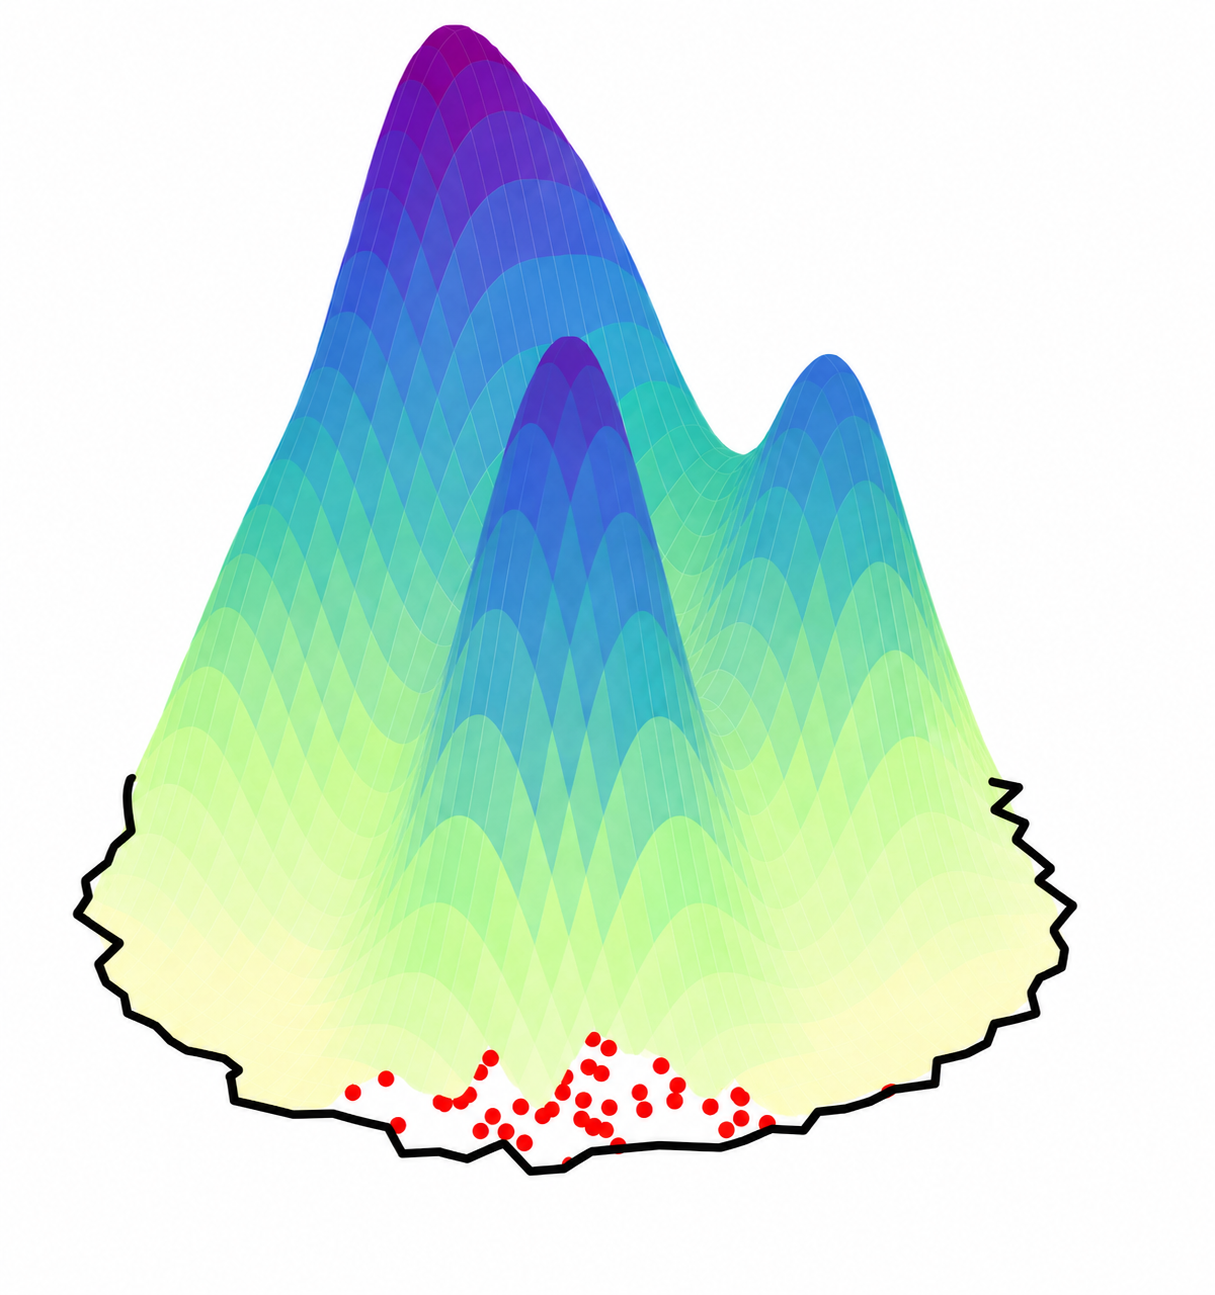
\includegraphics[width=0.3\linewidth]{plot.png}};

    % Title above image
    \hspace{-0.2cm}\node[anchor=south, font=\small\bfseries] at (img.north) {$P_\theta\big(\sigma \mid \sigma \in \mathcal{L}(G)\big)$};

    % Bottom-left label
    \node[
      anchor=south west,
      font=\small,
      fill=white,
      fill opacity=0.75,
      text opacity=1,
      inner sep=2pt
    ] at ([xshift=-0.4cm,yshift=0.03cm]img.south west)
      {$\mathcal{L}(G)$};
  \end{tikzpicture}
}